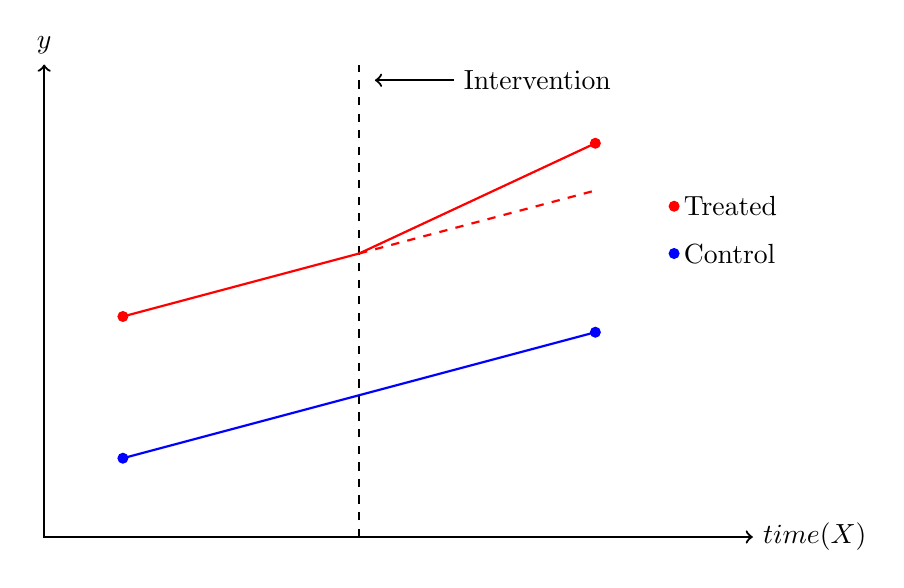
\begin{tikzpicture}[scale=2]
    
	% Draw axes
  \draw [<->,thick] (0,3) node (yaxis) [above] {$y$} |- (4.5,0) node (xaxis) [right] {$time (X)$};
	\draw[thick, color=black, dashed] (2,0) coordinate (t0_0) -- (2,3) coordinate (t0_1);
	
	% Legend
	\coordinate (T) at (4,2.1);
    \fill[red] (T) circle (1pt) node[right, color=black] {Treated};
	\coordinate (C) at (4,1.8);
    \fill[blue] (C) circle (1pt) node[right, color=black] {Control};
	
	% Intervention line
	\draw[thick, -> ] (2.6,2.9) coordinate (t0_0) node[right] {Intervention} -- (2.1,2.9) coordinate (t0_1);

    % control
	\draw[thick, color=blue] (0.5,0.5) coordinate (c0_0) -- (3.5,1.3) coordinate (c0_1);
    \fill[blue] (c0_0) circle (1pt);
    \fill[blue] (c0_1) circle (1pt);
    % treated
	\draw[thick, color=red] (0.5,1.4) coordinate (t0_0) -- (2.0,1.8) coordinate (t0_1);
	\draw[thick, color=red] (2.0,1.8) coordinate (t1_0) -- (3.5,2.5) coordinate (t1_1);
    \fill[red] (t0_0) circle (1pt);
    \fill[red] (t1_1) circle (1pt);
    % counterfactual
	\draw[thick, dashed, color=red] (2.0,1.8) coordinate (t1_0) -- (3.5,2.2) coordinate (t1_1);

\end{tikzpicture}